
\label{sec:theory_levels}

One fundamental part of all software development is the concept of
abstraction. Abstraction can be described as a way of decomposing an
application into different levels, with different level of detail. This
permits the developer to ignore certain details of the software, and
instead focus on other details. Consider the development of a simple
game with basic graphics: On a very low level, it requires a tremendous
amount of work in order to shuffle data between hardware buses, perform
memory accesses and CPU operations. By using higher abstraction levels,
one can use third-party frameworks for drawing graphics to the screen
and detecting collisions. The operating system and programming language
takes care of handling bus-accesses and memory management. This allows
the developer to focus on designing the game logic itself, rather than
bothering with drawing individual pixels or figuring out where in the
memory to store data. \cite{paper:abstraction}\\

In the same way, testing can be performed at several different levels.
There are several ways of defining these levels, but one way of
describing it is like a pyramid (\fref{fig:testing_pyramid}). We can
imagine testing at different levels as holding a flashlight at different
levels of the pyramid. If we hold the flashlight at the top of the
pyramid, the flashlight will illuminate a large part of the pyramid. If
the flashlight is hold at the bottom of the pyramid, a much smaller
piece of the pyramid will be illuminated. Similar to this, testing at a
high level permits us to ignore a lot of details. Due to the high level
of abstraction, a large part of the code must be run in order for the
test to be completed. Testing at a lower level requires a much smaller part
of the code to be run. Different levels of testing have different
advantages, drawbacks and uses, which will be covered in the following
subsections.\\

\begin{figure}
\centering
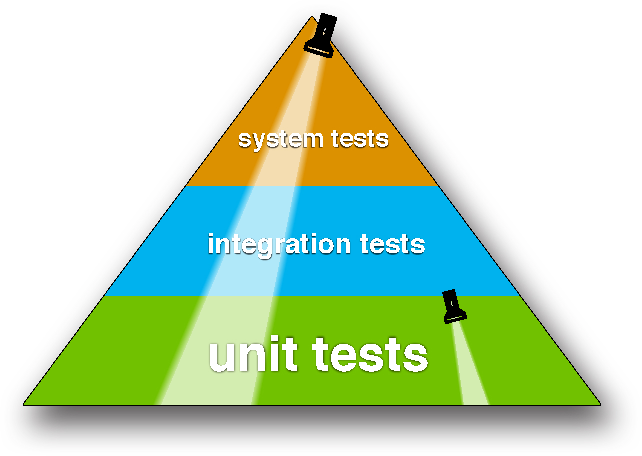
\includegraphics[width=0.7\textwidth]{theory/levels/triangle}
\caption{The software testing pyramid, with two flashlights at different
         levels illustrating how the level of testing affects the amount
         of tested code.}
\label{fig:testing_pyramid}
\end{figure}
